\let\negmedspace\undefined
\let\negthickspace\undefined
\documentclass[journal]{IEEEtran}
\usepackage[a5paper, margin=10mm, onecolumn]{geometry}
\usepackage{lmodern} 
\usepackage{tfrupee} 

\setlength{\headheight}{1cm} % Set the height of the header box
\setlength{\headsep}{0mm}     % Set the distance between the header box and the top of the text

\usepackage{gvv-book}
\usepackage{gvv}
\usepackage{cite}
\usepackage{amsmath,amssymb,amsfonts,amsthm}
\usepackage{algorithmic}
\usepackage{graphicx}
\usepackage{textcomp}
\usepackage{xcolor}
\usepackage{txfonts}
\usepackage{listings}
\usepackage{enumitem}
\usepackage{mathtools}
\usepackage{gensymb}
\usepackage{comment}
\usepackage[breaklinks=true]{hyperref}
\usepackage{tkz-euclide} 
\usepackage{listings}                                      
\def\inputGnumericTable{}                                 
\usepackage[latin1]{inputenc}                                
\usepackage{color}                                            
\usepackage{array}                                            
\usepackage{longtable}
\usepackage{multicol}
\usepackage{calc}                                             
\usepackage{multirow}                                         
\usepackage{hhline}                                           
\usepackage{ifthen}                                           
\usepackage{lscape}
\begin{document}

\bibliographystyle{IEEEtran}
\vspace{3cm}

\title{4.7.22}
\author {EE25BTECH11031 - Sai Sreevallabh}
% \maketitle
% \newpage
% \bigskip
{\let\newpage\relax\maketitle}

\renewcommand{\thefigure}{\theenumi}
\renewcommand{\thetable}{\theenumi}
\setlength{\intextsep}{10pt} % Space between text and floats


\numberwithin{equation}{enumi}
\numberwithin{figure}{enumi}
\renewcommand{\thetable}{\theenumi}

\textbf{Question: }\\

In what direction should a line be drawn through the point $\brak{1,2}$ so that its point of intersection with the line $x+y=4$ is at a distance $\sqrt{63}$\\

\textbf{Solution: }\\

The given point is $\vec{P} = \myvec{1\\2}$.\\

The given line can be represented as $\vec{n}^\top\vec{x} = c$, where 
\begin{align}
    \vec{n} = \myvec{1\\1} \ \ c = 4
\end{align}\\

A parametric point on the line passing through the point $\vec{P}$ is given by 
\begin{align}
    \vec{r} = \vec{P} + \lambda\vec{m}
\end{align}

where $\vec{m} = \myvec{1\\m}$\\

Plugging in the parametric form of the point in the line equation, we get: 

\begin{align}
    \vec{n}^\top\brak{\vec{P+\lambda\vec{m}}} =&\  c\\
    \lambda =& \frac{c-\vec{n}^\top\vec{P}}{\vec{n}^\top\vec{m}}
\end{align}\\

Replacing this value of $\lambda$ in the equation of the parametric point, we get it to be
\begin{align}
    \vec{r} = \vec{P} + \brak{\frac{c-\vec{n}^\top\vec{P}}{\vec{n}^\top\vec{m}}}\vec{m}
\end{align}\\

Let the distance between this point and $\vec{P}$ be $d = \sqrt{63}$. 
\begin{align}
    d = \norm{\vec{r} - \vec{P}}
\end{align}

\begin{align}
    d = \abs{\frac{c-\vec{n}^\top\vec{P}}{\vec{n}^\top\vec{m}}}\norm{\vec{m}}
\end{align}

Substituting the values, we get

\begin{align}
    \sqrt{63} =& \abs{\frac{4-3}{1+m}}\sqrt{1+m^2}
\end{align}\\

Squaring on both sides:
\begin{align}
    63 =& \frac{1+m^2}{\brak{1+m}^2}
\end{align}

This is an equation in $m$. Upon solving this equation, we get:

\begin{align}
    m = \frac{-63 \pm 5\sqrt{5}}{62}
\end{align}

$\therefore$ The direction vector $\vec{m}$ can take two values:
\begin{center}
    $\vec{m} = \myvec{1\\\frac{-63 + 5\sqrt{5}}{62}} \ \ \text{or} \ \ \vec{m} = \myvec{1\\\frac{-63 - 5\sqrt{5}}{62}}$
\end{center}

\begin{figure}[H]
    \centering
    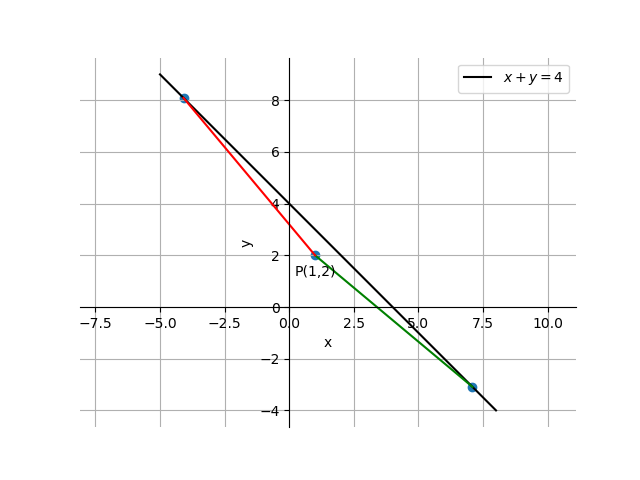
\includegraphics[width=0.9\linewidth]{Figs/plot(py+C).png}
\end{figure}
\end{document}\
